\section{Methodology}

\begin{frame}{The DeCoR Algorithm}
    \begin{block}{Algorithm 1: Deconfounding via Robust Regression}

        \hrule
        \vspace{0.1cm}
        \textbf{Require:} $X^n \in \mathbb{R}^{n \times d}$, $Y^n \in \mathbb{R}^n$, orthonormal basis $\phi$, robust linear regression algorithm $\mathcal{A}$
        
        \begin{center}
            \begin{tabular}{l l}
                $X_\phi^n \leftarrow (T_1^{\phi,n}(X), \dots, T_n^{\phi,n}(X))^\top$ & \textcolor{blue}{$\triangleright$ Translate to frequency domain}\\
                $Y_\phi^n \leftarrow (T_1^{\phi,n}(Y), \dots, T_n^{\phi,n}(Y))^\top$  \\
                $\hat{\beta}_{\text{DeCoR}}^{\phi,n} \leftarrow \mathcal{A}(X_\phi^n, Y_\phi^n)$ &  \textcolor{blue}{$\triangleright$ robust regression} \\
                \textbf{return} $\hat{\beta}_{\text{DeCoR}}^{\phi,n}$ & 
            \end{tabular}
        \end{center}
        
        \hrule

    \end{block}

    \textbf{Insights:}
        \begin{itemize}
            \item \textbf{Modular Design:} Complexity shifted to the transformation step ($T^{\phi,n}$).
            \item \textbf{Flexible basis:} Requires only an orthonormal basis $\phi$ (e.g., Cosine).
            \item \textbf{Plug-and-play solver:} Uses any standard robust regression algorithm $\mathcal{A}$.
        \end{itemize}
\end{frame}

\begin{frame}{The Torrent Algorithm \cite{bhatia2015robustregressionhardthresholding}}
    \begin{block}{Algorithm 3: Torrent (Bhatia et al., 2015)}
        \vspace{0.1cm}
        \hrule
        \vspace{0.1cm}
        \begin{tabular}{l l}
            \multicolumn{2}{l}{\textbf{Require} $X \in \mathbb{R}^{n \times d}$, $Y \in \mathbb{R}^n$, $a \in \{1, \dots, n\}$} \\
            \multicolumn{2}{l}{$S_0 \leftarrow \{1, \dots, n\}, e \leftarrow Y, \text{err} \leftarrow \infty, t \leftarrow 0$} \\
            \multicolumn{2}{l}{\textbf{while} $\|e\|_2 < \text{err}$ \textbf{do}} \\
            \hspace{0.5cm} $t \leftarrow t + 1$ & \\
            \hspace{0.5cm} $\text{err} \leftarrow \|e\|_2$ & \\
            \hspace{0.5cm} $\hat{\beta}_{\text{Tor}}^t \leftarrow \hat{\beta}_{\text{OLS}}^{S_{t-1}}(X, Y)$ & \textcolor{blue}{$\triangleright$ Fit OLS on subset $S_{t-1}$ from prev. iteration}\\
            \hspace{0.5cm} $v \leftarrow |Y - X\hat{\beta}_{\text{Tor}}^t|$ & \textcolor{blue}{$\triangleright$ Calc residuals for ALL data points} \\
            \hspace{0.5cm} $S_t \leftarrow \text{HT}(v, a)$ & \textcolor{blue}{$\triangleright$ Keep $a$ many points with smallest residuals} \\
            \hspace{0.5cm} $e \leftarrow |Y_{S_t} - X_{S_t}\hat{\beta}_{\text{Tor}}^t|$ & \textcolor{blue}{$\triangleright$ Measure error on the new clean subset $S_t$} \\
            \multicolumn{2}{l}{\textbf{end while}} \\
            \multicolumn{2}{l}{\textbf{return} $\hat{\beta}_{\text{Tor}}^{n,a} := \hat{\beta}_{\text{Tor}}^t$} 
        \end{tabular}
        \vspace{0.1cm}
        \hrule
        \vspace{0.1cm}
    \end{block}
\end{frame}

\begin{frame}
        \begin{figure}
        \centering
        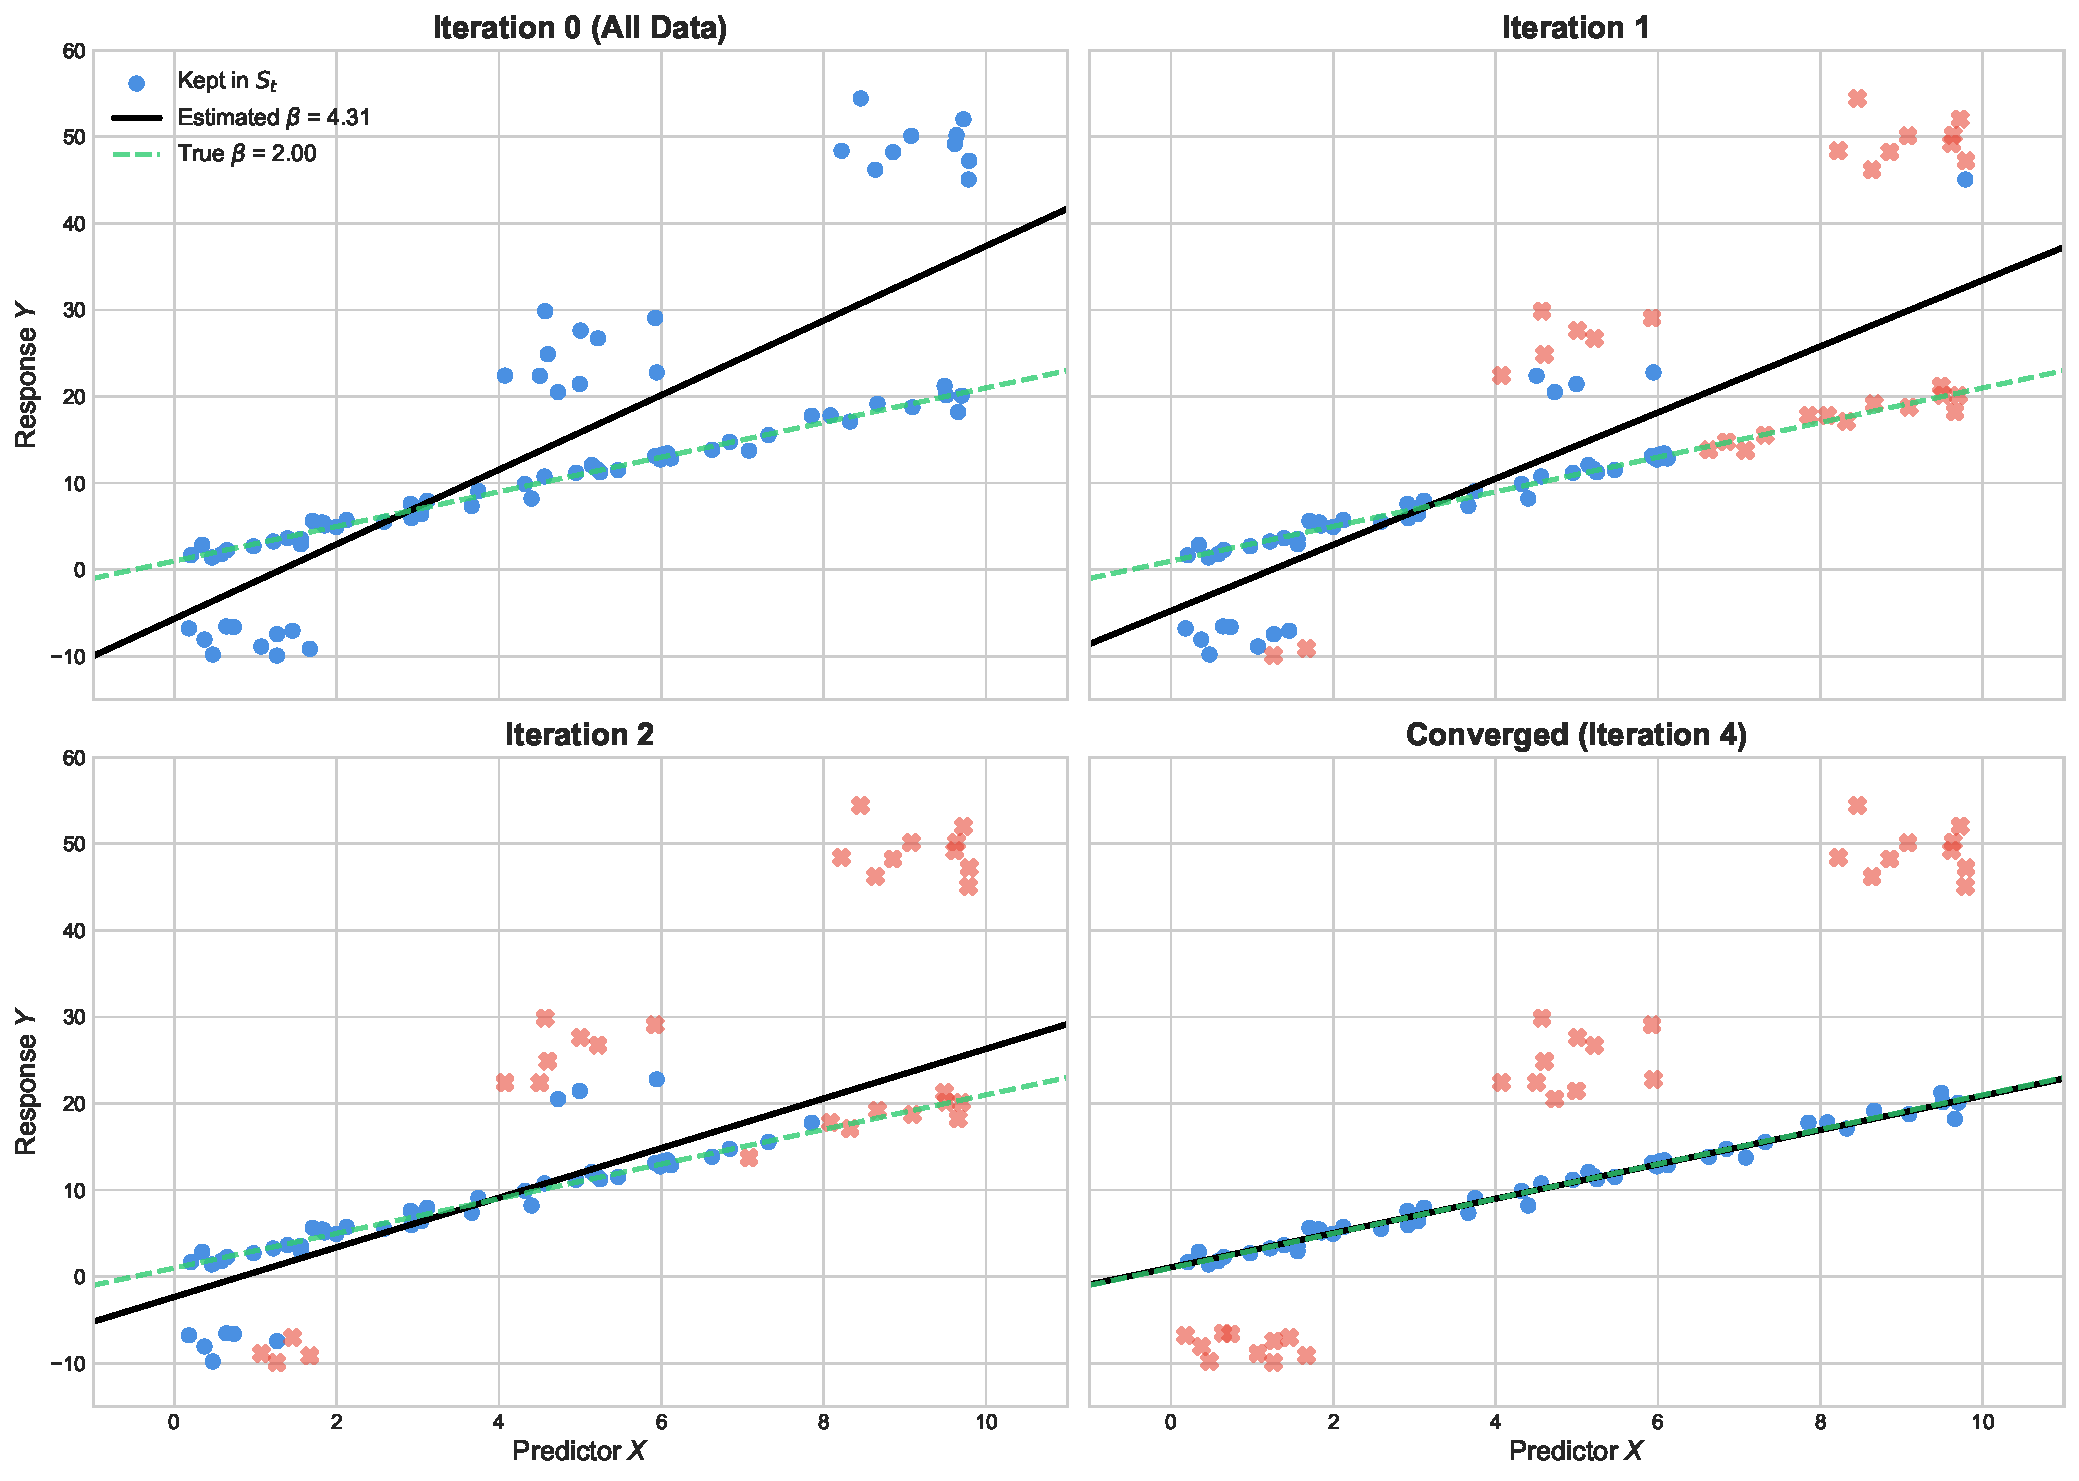
\includegraphics[width=\textwidth]{figures/methodology/torrent_convergence.pdf}
    \end{figure}
\end{frame}

\begin{frame}{Empirical Convergence of Torrent}

    \begin{table}
        \centering
        % Increase row height slightly for better readability on a projector
        \renewcommand{\arraystretch}{1.3} 
        \begin{tabular}{|c|c|c|c|}
            \hline
            \textbf{$n$} & \textbf{mean} & \textbf{min} & \textbf{max} \\
            \hline
            10   & 2.42 & 2 & 3  \\
            100  & 5.14 & 3 & 8  \\
            1000 & 8.26 & 4 & 13 \\
            \hline
        \end{tabular}
    \end{table}

    \vspace{0.5cm}

    \begin{block}{Convergence Speed}
        Even for a large sample size of $n = 1000$, Torrent converges in \textbf{$< 15$ iterations}.
    \end{block}
    \textbf{Experimental setting:} $X$ and $U$ are band-limited processes, theshold param. $a = 0.7$, elements of $G_n$ chosen uniformly at random with probability 0.25 \cite{schur2024decordeconfoundingtimeseries}. 

\end{frame}